%% 
%% Copyright 2019-2020 Elsevier Ltd
%% 
%% This file is part of the 'CAS Bundle'.
%% --------------------------------------
%% 
%% It may be distributed under the conditions of the LaTeX Project Public
%% License, either version 1.2 of this license or (at your option) any
%% later version.  The latest version of this license is in
%%    http://www.latex-project.org/lppl.txt
%% and version 1.2 or later is part of all distributions of LaTeX
%% version 1999/12/01 or later.
%% 
%% The list of all files belonging to the 'CAS Bundle' is
%% given in the file `manifest.txt'.
%% 
%% Template article for cas-dc documentclass for 
%% double column output.

% \documentclass[a4paper,fleqn]{cas-dc}
\documentclass[a4paper,fleqn]{DC_ArtStyle}
% \documentclass[]{interact}

% \usepackage[authoryear,longnamesfirst]{natbib}
% \usepackage[authoryear]{natbib}
\usepackage[numbers]{natbib}
\usepackage{lipsum}
\usepackage{xcolor}
\usepackage{caption}
\usepackage{subcaption}
\usepackage{siunitx}
\usepackage{array}
\usepackage{multirow}
\usepackage{amsmath}
\usepackage{amssymb}
\usepackage{rotating}
\usepackage{float}
\usepackage{multicol}
\usepackage{pdfpages}
\usepackage[normalem]{ulem}
\usepackage[justification=centering]{caption}
\usepackage{cuted}


\newcommand{\abbreviations}[1]{%
	\nonumnote{\textit{Abbreviations:\enspace}#1}}

\setlength{\parindent}{0pt}

\begin{document}
	\let\WriteBookmarks\relax
	\def\floatpagepagefraction{1}
	\def\textpagefraction{.001}
	\shorttitle{Fabric-Elasticity Property Relationships of the Human Cortical Femur}
	\shortauthors{Simon et~al.}
	
	\title[mode = title]{Fabric-Elasticity Property Relationships of the Human Cortical Femur}
	
	% Autors
	\author{Mathieu Simon}
	\ead{mathieu.simon@artorg.unibe.ch}

    \author{Gabriela Gerber}
    
    \author{Simone Poncioni}

	\author{Yvan Gugler}

	\author{Kurt Lippuner}

	\author{Philippe Zysset}
	\ead{philippe.zysset@artorg.unibe.ch}

	
	% Adresses
	\address{ARTORG Centre for Biomedical Engineering Research, University of Bern, Bern, Switzerland}
	
	% Abbreviations
	\abbreviations{%
		ROI, region of interest;
		\textmu CT, micro-computed tomography;
		}
	
	% Footnotes
	
	%
	%
	%
	% ABSTRACT
	%
	%
	%
	
	\begin{abstract}
		Lorem ipsum dolor sit amet, consectetuer adipiscing elit.
		Utpurus elit, vestibulum ut, placerat ac, adipiscing vitae, felis.
		Curabitur dictum gravida mauris.
		Nam arcu libero, nonummy eget, consectetuer id, vulputate a, magna.
		Donec vehicula augue eu neque.
		Pellentesque habitant morbi tristique senectus et netus et malesuada fames ac turpis egestas.
		Mauris ut leo. Cras viverra metus rhoncus sem.
		\\[0.5em]
		Nulla et ectus vestibulum urna fringilla ultrices.
		Phasellus eu tellus	sit amet tortor gravida placerat.
		Integer sapien est, iaculis	in, pretium quis, viverra ac, nunc.
		Praesent eget sem vel leo ultrices bibendum.
		Aenean faucibus. Morbi dolor nulla,	malesuada eu, pulvinar at, mollis ac, nulla.
		Curabitur auctor semper nulla.
		Donec varius orci eget risus.
		Duis nibh mi, congue eu, accumsan eleifend, sagittis quis, diam.
		Duis eget orci sit amet orci dignissim rutrum.
		\\[0.5em]
		Nam dui ligula, fringilla a, euismod sodales, sollicitudin vel, wisi.
		Morbi auctor lorem non justo.
		Nam lacus libero, pretium at, lobortis vitae, ultricies et, tellus.
		Donec aliquet, tortor sed accumsan bibendum, erat ligula aliquet magna, vitae ornare odio metus a mi.
		Morbi ac orci et nisl hendrerit mollis.
		Suspendisse ut massa.
		Cras nec ante.
		Pellentesque a nulla.
		Cum sociis natoque penatibus et magnis dis parturient montes, nascetur ridiculus mus.
		Aliquam tincidunt urna.
		Nulla ullamcorper vestibulum turpis.
		Pellentesque cursus luctus mauris.
    \end{abstract}
	
	\begin{keywords}
		Bone \sep%
		Fabric \sep%
		Elasticity \sep%
	\end{keywords}
	

	\begin{NoHyper}
		\maketitle
	\end{NoHyper}
	
	%
	%
	%
	% INTRO
	%
	%
	%
	
	\section{Introduction}
	Bone is a hierarchical material\dots
	\subsection{Bone structure}
	\begin{itemize}
		\item Bone composition
		\item Mineralised collagen fibrils
		\item Lamellar bone
		\item Osteon
		\item Cortical bone
	\end{itemize}
	\subsection{Mechanical testing}
	\begin{itemize}
		\item Nanoindentation
		\item Resonant ultrasound spectroscopy
	\end{itemize}
	\subsection{Imaging}
	\begin{itemize}
		\item Micro-computed tomography
	\end{itemize}
	\subsection{Bone Properties Estimation}
	\begin{itemize}
		\item Micro finite element analysis
		\item Density and fabric
		\item Homogenised finite element analysis
	\end{itemize}
	The aim of the present study is to investigate the influence of the bone matrix properties and microstructure on the mechanical properties of human bone.
	The relationships between density, fabric and mechanics are presented from the bone matrix (bone of full density) down to the low density of trabecular bone with a strong focus on the cortical bone.
	Additionally to relationships description, the ojective is to provide material constants for bone properties estimation.

	%
	%
	%
	% METHODS
	%
	%
	%
	
	\newpage
	\section{Material and Methods}

	\subsection{Bone Experimental Properties}
	Lamellar bone
	\begin{itemize}
		\item Nanoindentation data
		\item Virtual fabric
	\end{itemize}

	Cortical bone
	\begin{itemize}
		\item Samples
		\item Micro-CT
		\item RUS data
	\end{itemize}

	In the present study:
	\begin{itemize}
		\item Downsampling factor 2
		\item 16x 1mm\textsuperscript{3} Relationships
		\item Isotropic vs transverse isotropic material
		\item Average $\mathbb{S}$ per sample
	\end{itemize}

	\begin{figure}[!h]
		\centering
		\begin{subfigure}[t]{.45\linewidth}
			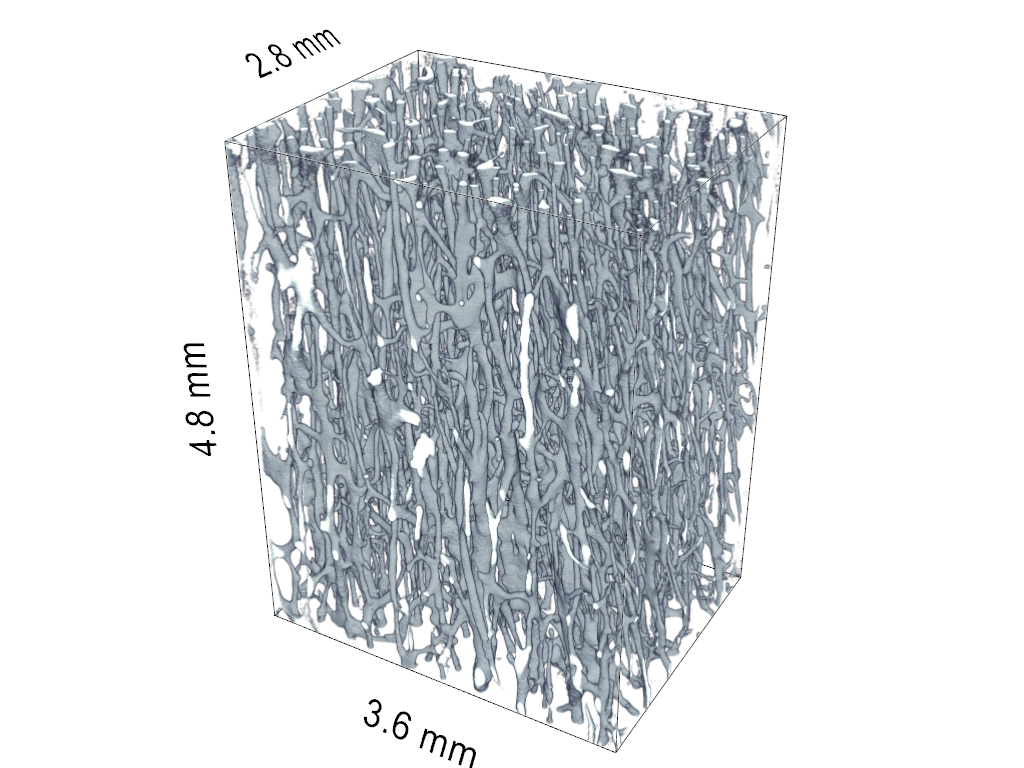
\includegraphics[height=0.8\linewidth]{../_Results/Cortical/Scans/2009_213_L}
			\caption{Typical sample with its porosities}
		\end{subfigure}
		\begin{subfigure}[t]{0.45\linewidth}
			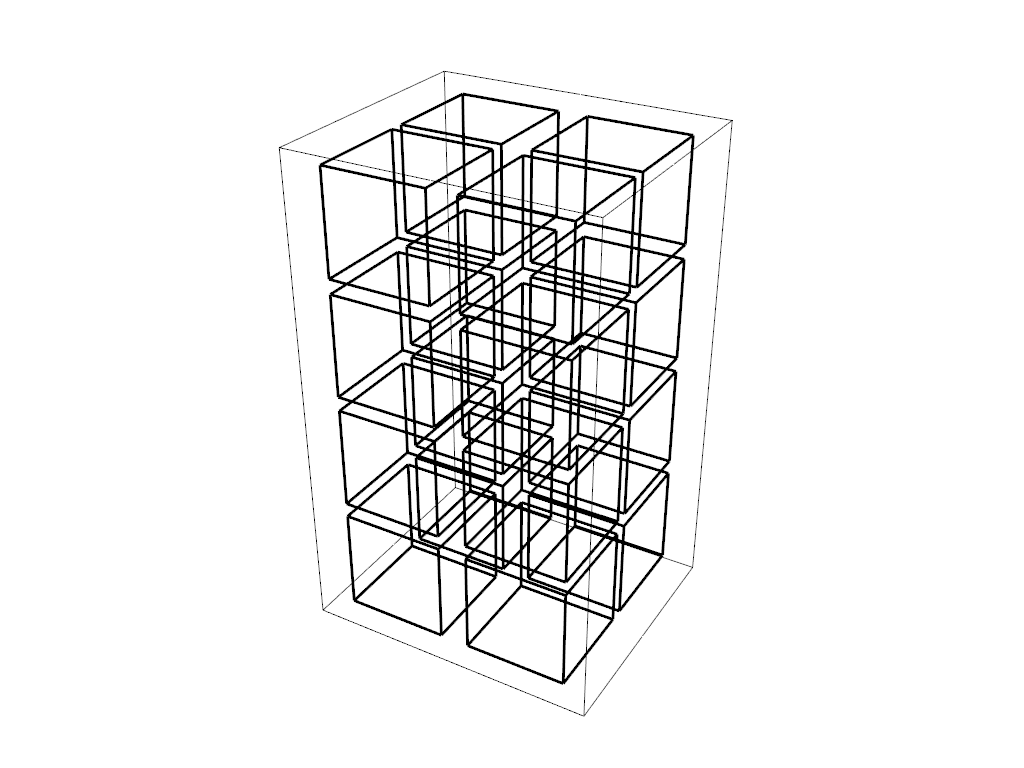
\includegraphics[height=0.8\linewidth, trim=50 50 50 0]{../_Results/Cortical/ROIs/ROIs}
			\caption{ROIs analysed}
		\end{subfigure}
	\end{figure}

	\subsection{Theorical Model}
	\begin{itemize}
		\item Density-elasticity relationships
		\item Fabric-elasticity relationships
	\end{itemize}

	Proposed Model
	Hypotheses:
	\begin{itemize}
		\item Cortical bone: $\rho$ > 0.5
		\item Transverse isotropic: m1 = m2
		\item Homogeneous samples: CV < 0.263
	\end{itemize}
	\begin{equation}
		\mathbf{S} = \sum_{i=1}^{6} \Lambda_{i} \mathbf{N}_i \otimes \mathbf{N}_i\\
	\end{equation}

	Project to transverse isotropy
	\begin{equation}
		\mathbf{S} =
		\begin{pmatrix}
			S_{11} & S_{12}^T & S_{13}^T & 0 & 0 & 0 \\
			S_{21} & S_{22}^T & S_{23}^T & 0 & 0 & 0 \\
			S_{31} & S_{32}^T & S_{33}^T & 0 & 0 & 0 \\
			0 & 0 & 0 & S_{44}^T & 0 & 0 \\
			0 & 0 & 0 & 0 & S_{55}^T & 0 \\
			0 & 0 & 0 & 0 & 0 & S_{66}^T \\
		\end{pmatrix}
	\end{equation}

	\begin{equation}
		\mathbf{S}_{transverse} =
		\begin{pmatrix}
			S'_{11} & S'_{12} & S'_{13} & 0 & 0 & 0 \\
			S'_{12} & S'_{22} & S'_{23} & 0 & 0 & 0 \\
			S'_{13} & S'_{23} & S'_{33} & 0 & 0 & 0 \\
			0 & 0 & 0 & S'_{44} & 0 & 0 \\
			0 & 0 & 0 & 0 & S'_{55} & 0 \\
			0 & 0 & 0 & 0 & 0 & S_{66} \\
		\end{pmatrix}
	\end{equation}

	\begin{equation}
		\begin{pmatrix}
		S_{11} \\
		S_{12} \\
		S_{13} \\
		S_{21} \\
		S_{22} \\
		S_{23} \\
		S_{31} \\
		S_{32} \\
		S_{33} \\
		S_{44} \\
		S_{55} \\
		S_{66} \\
		\end{pmatrix} = \begin{pmatrix}
		1 & 0 & 0 & 0 & 0\\
		0 & 1 & 0 & 0 & 0\\
		0 & 0 & 1 & 0 & 0\\
		0 & 1 & 0 & 0 & 0\\
		1 & 0 & 0 & 0 & 0\\
		0 & 0 & 1 & 0 & 0\\
		0 & 0 & 1 & 0 & 0\\
		0 & 0 & 1 & 0 & 0\\
		0 & 0 & 0 & 1 & 0\\
		0 & 0 & 0 & 0 & 1\\
		0 & 0 & 0 & 0 & 1\\
		1 &-1 & 0 & 0 & 0\\
		\end{pmatrix} \begin{pmatrix}
		S'_{11} \\
		S'_{12} \\
		S'_{13} \\
		S'_{33} \\
		S'_{44} \\
		\end{pmatrix}
		\label{EqFit}
	\end{equation}
	
	%
	%
	%
	% RESULTS
	%
	%
	%

	\clearpage
	\section{Results}
	\subsection{Nanoindentation}
	\begin{table*}
		\caption{Nanoindentation - cortical bone matrix properties}
		\resizebox{\linewidth}{!}{%
		\begin{tabular}{l|c|c|c|c|c|c|c|c|c}
			Study & E1 & E2 & E3 & Nu12 & Nu13 & Nu23 & Mu12 & M13 & Mu23 \\
			\hline
			Dall'Ara & & & & & & & & & \\
			Fanzoso  & & & & & & & & & \\
			Present  & 14796.9 & 14796.9 & 21175.8 & 0.34 & 0.284214 & 0.284214 & 5521.23 & 6604.96 & 6604.96 \\
			\hline
		\end{tabular}}
	\end{table*}

	\subsection{Cortical Bone Morphology}
	\begin{figure}
		\centering
			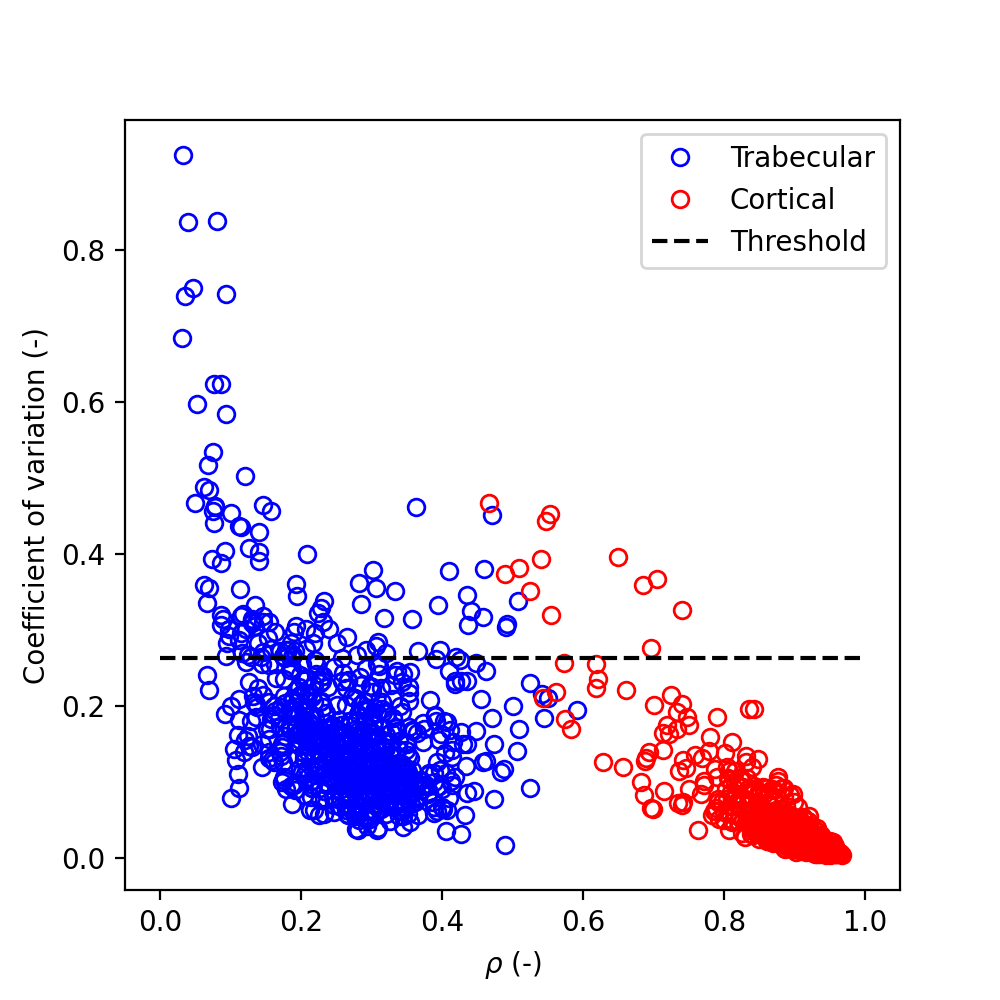
\includegraphics[width=\linewidth]{../_Results/Cortical/CV_Rho}
			\caption{Coefficient of variation as function of porosity}
	\end{figure}
	\begin{figure*}
		\centering
		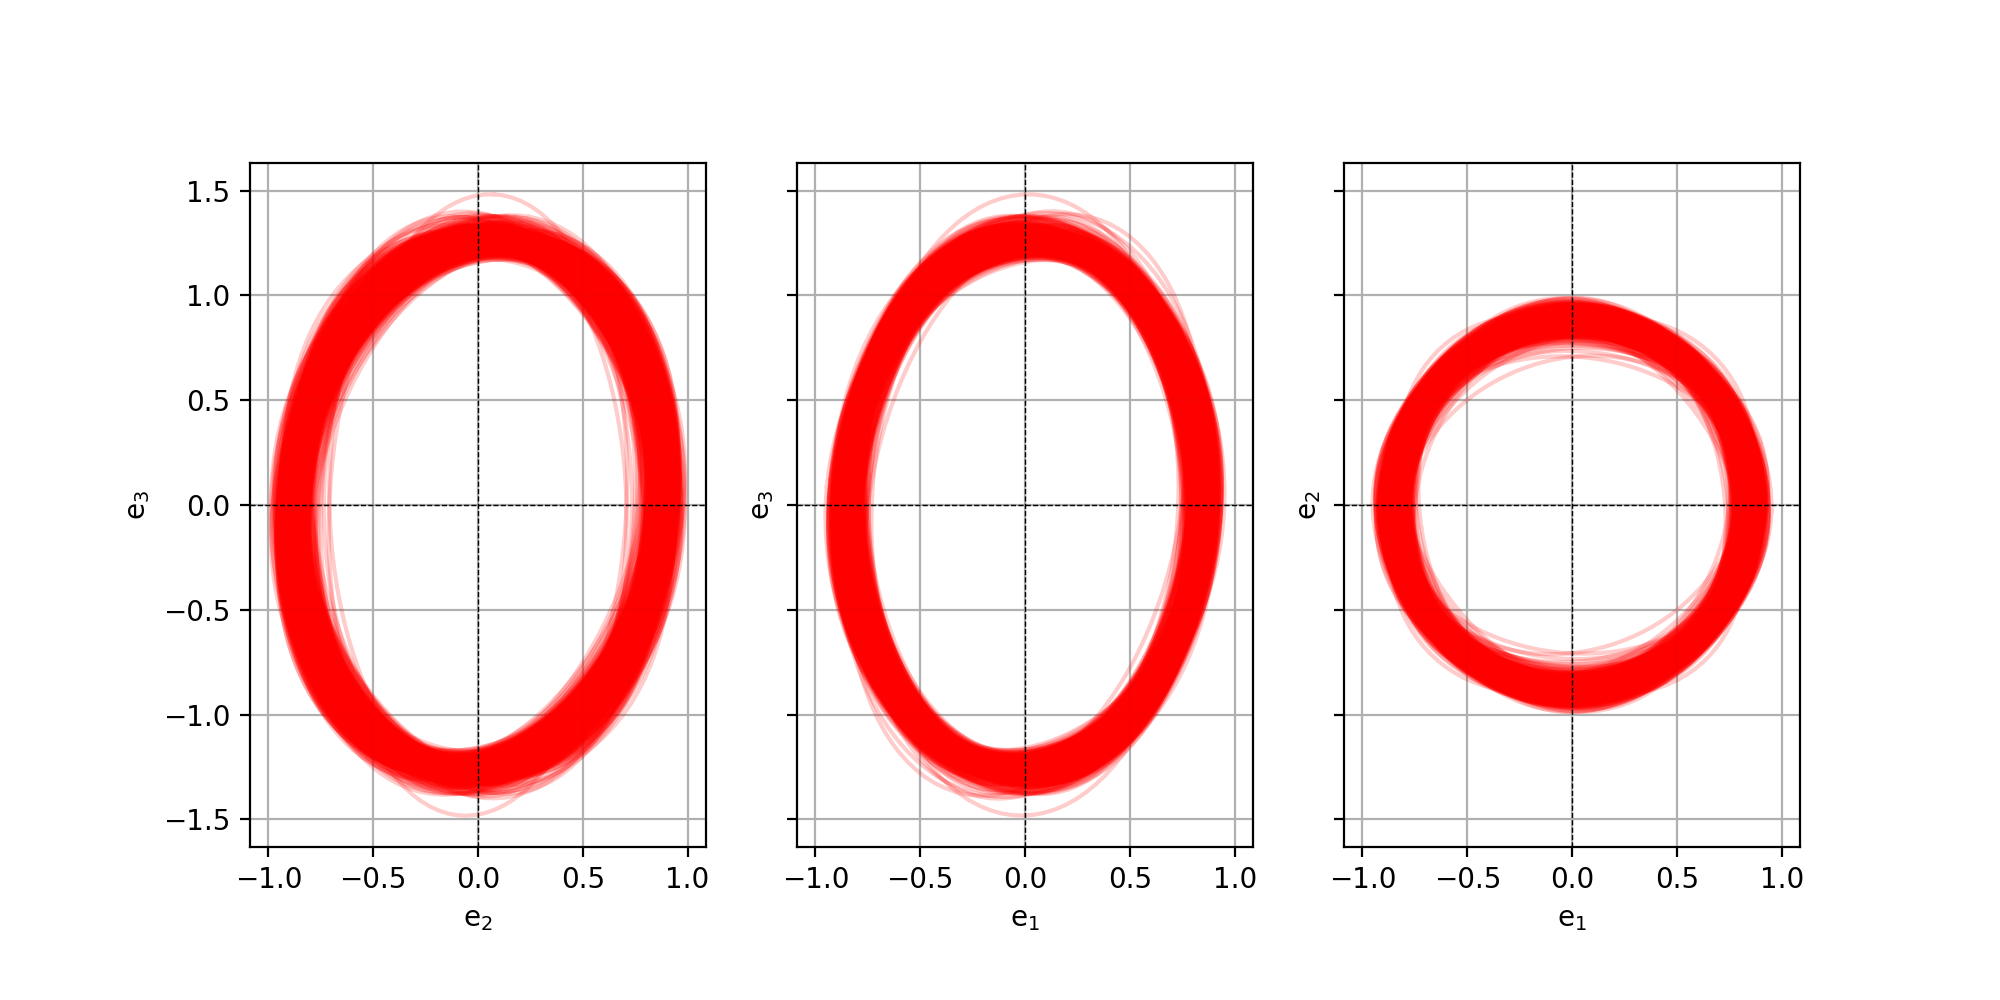
\includegraphics[width=\linewidth]{../_Results/Cortical/Fabric/Fabric}
		\caption{ROIs fabric projected on principal planes}
	\end{figure*}
	
	\clearpage
	\subsection{Fit to model}
	\begin{figure*}
		\centering
		\begin{subfigure}[t]{.45\linewidth}
			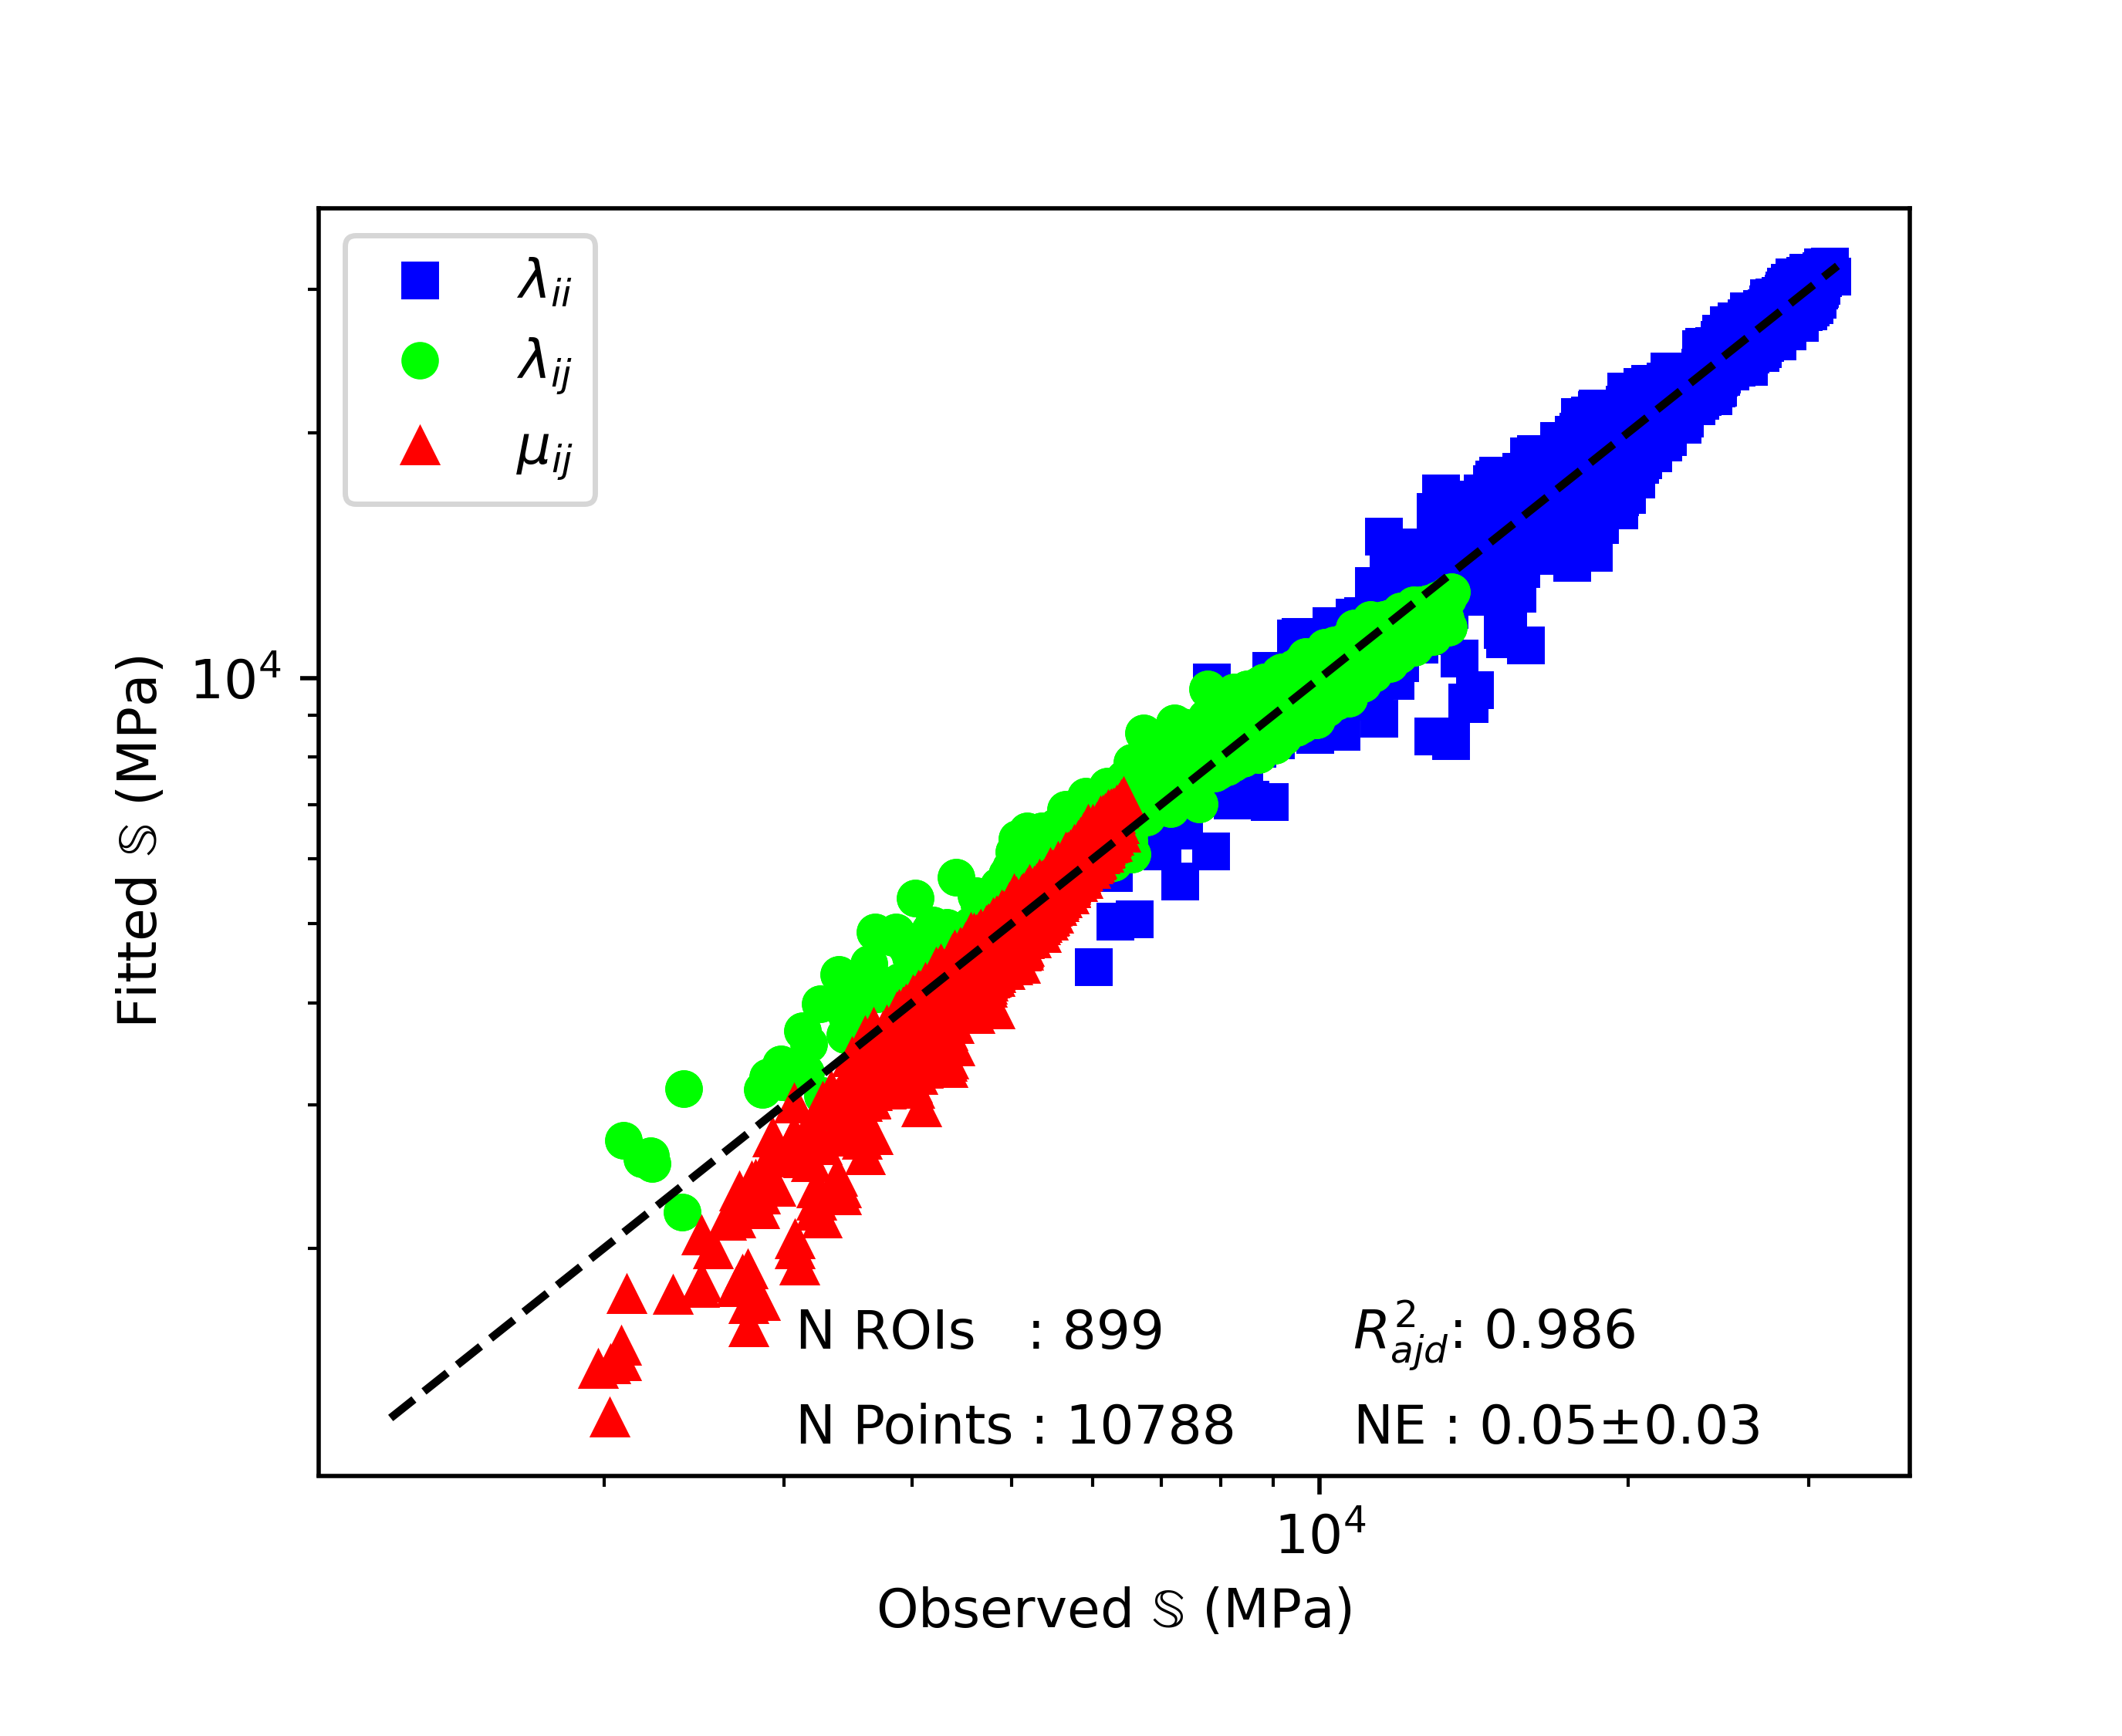
\includegraphics[height=0.8\linewidth]{../_Results/StandardOrthoModel}
			\caption{Orthotropic space}
		\end{subfigure}
		\begin{subfigure}[t]{.45\linewidth}
			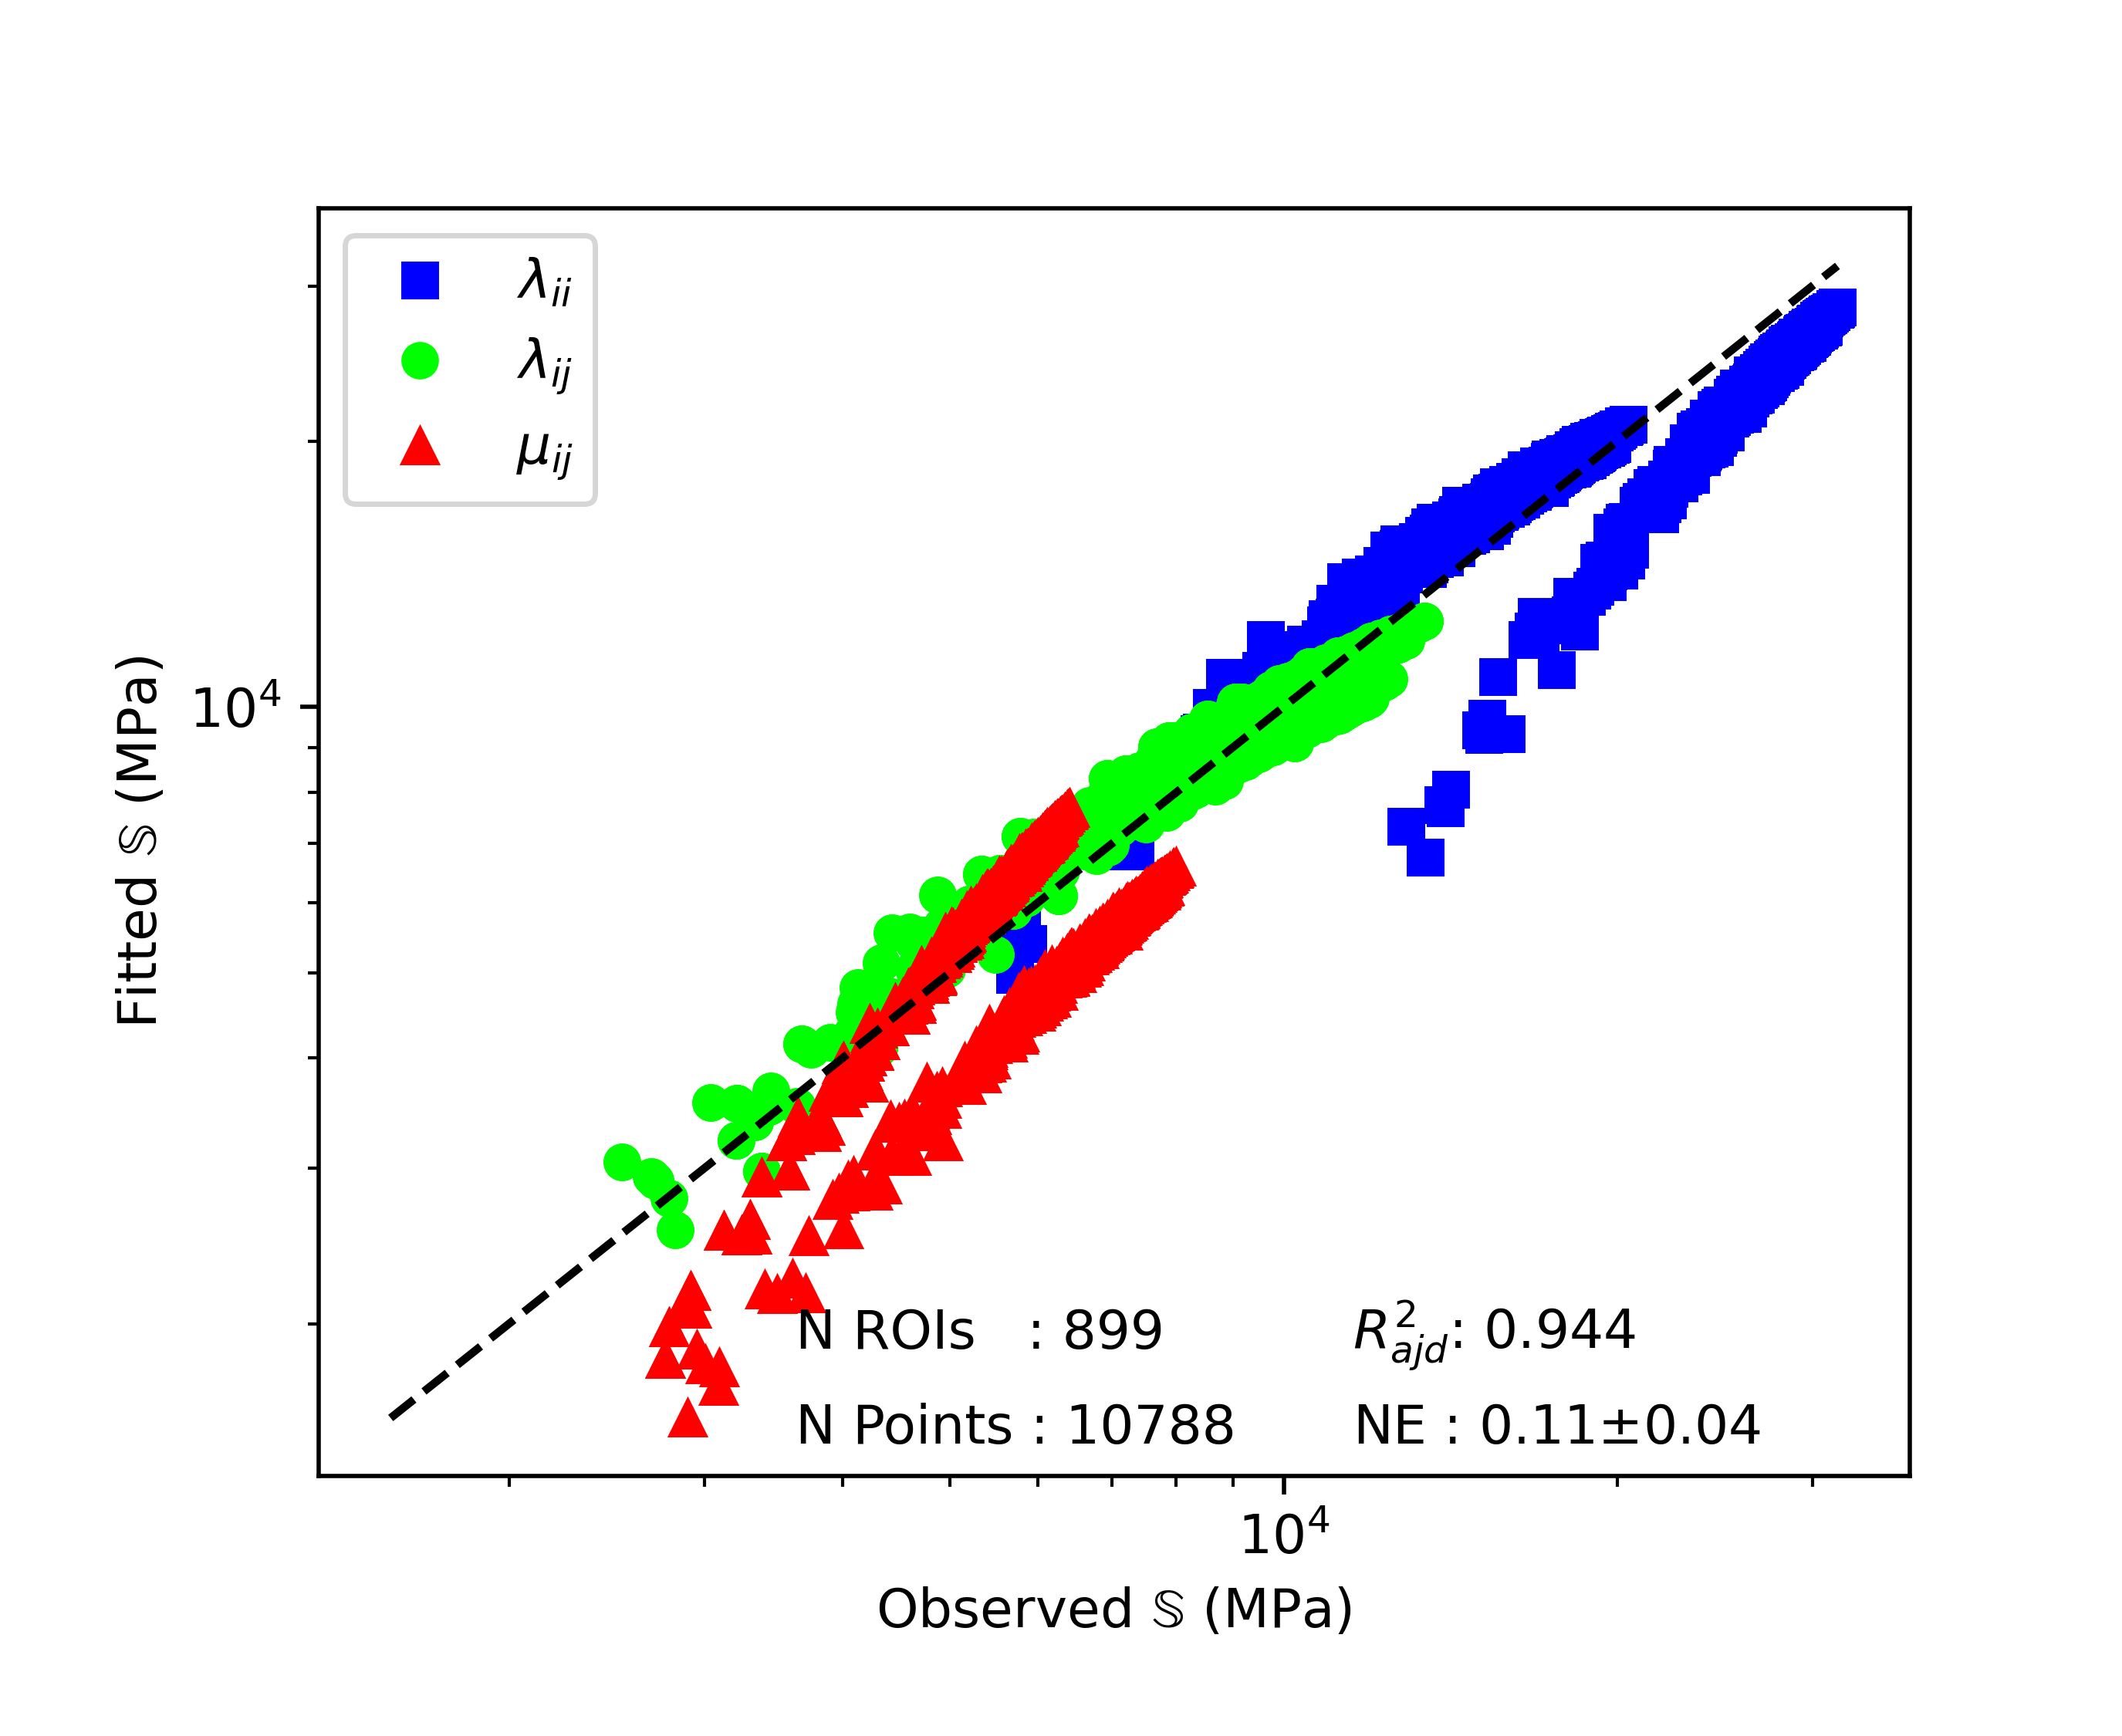
\includegraphics[height=0.8\linewidth]{../_Results/StandardTransModel}
			\caption{Transverse isotropic space}
		\end{subfigure}
		\caption{Fit to Zysset-Curnier model}
	\end{figure*}
	\begin{table}[!h]
		\centering
		\caption{Parameters and fit quality coefficient obtained with the standard Zysset-Curnier model in orthotropic and transverse isotropic space.}
		\label{TabZysset}
		\begin{tabular}{l|c|c|c|c|c|c|c}
		\toprule
			Model & $\lambda_0$ & $\lambda_0'$ & $\mu_0$ &  $k$ &  $l$ & $R^2_{adj}$ &   NE \\
		\midrule
		Orthotropic &       19831 &        12618 &    3527 & 2.48 & 0.57 &        0.99 & 0.05 \\
		Transverse &       12901 &        13234 &    6432 & 2.49 & 0.65 &        0.94 & 0.07 \\
		\bottomrule
		\end{tabular}
	\end{table}

	\begin{figure*}
		\centering
			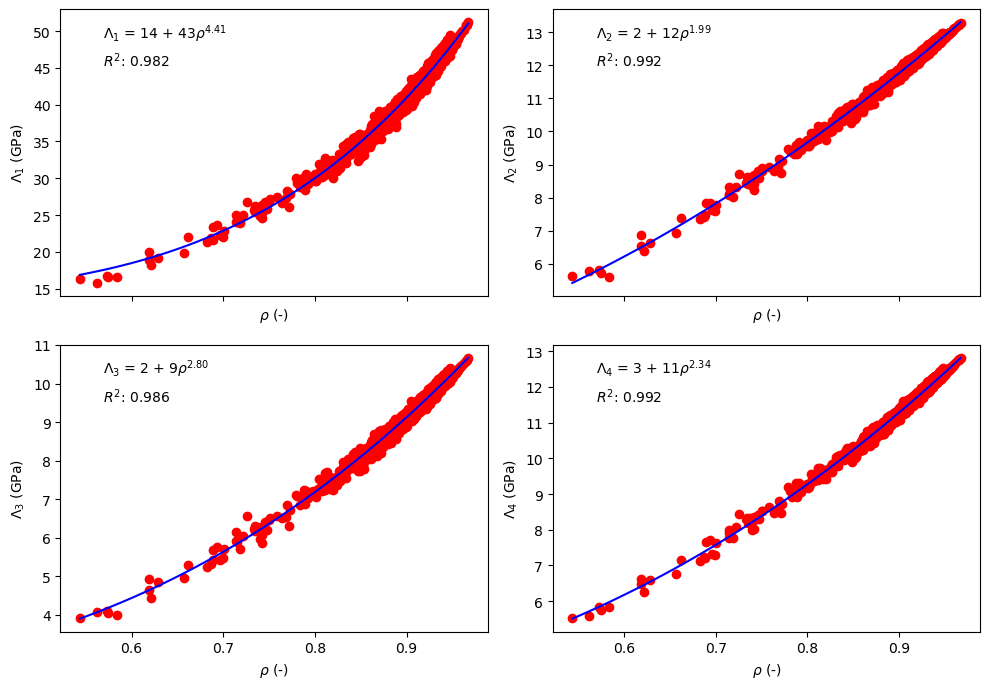
\includegraphics[width=\linewidth]{../_Results/CowinModel}
			\caption{Fit to Yang and Cowin model}
	\end{figure*}

	% \begin{table*}[!h]
	% 	\resizebox{\linewidth}{!}{%
	% 	\begin{tabular}{l|c|c|c|c|c|c|c|c|c|c|c|c|c|c|c|c}
	% 		Model & $\lambda_0$ & $\lambda_0$' & $\mu_0$ & $k_{\lambda_{11}}$ & $k_{\lambda_{22}}$ & $k_{\lambda_{33}}$ & $k_{\lambda_{12}}$ & $k_{\lambda_{31}}$ & $k_{\lambda_{23}}$ & $k_{\mu_{12}}$ & $k_{\mu_{31}}$ & $k_{\mu_{23}}$ & $l$ & $R^2_{adj}$ & NE \\
	% 		\hline
	% 		Alternative k & 19395 & 13126 & 3179 & 2.36 & 2.24 & 1.77 & 2.84 & 2.76 & 2.84 & 1.54 & 1.60 & 1.72 & 0.53 & 0.995 & 0.03 \\
	% 		Proposed l & 21329 & 13014 & 3200 & 3.12 & 3.12 & 2.12 & 3.12 & 2.62 & 2.62 & 1.92 & 1.61 & 1.61 & 0.44 & 0.988 & 0.05 \\
	% 		\hline
	% 	\end{tabular}}
	% \end{table*}

	% \clearpage
	% \subsection{Connection to trabecular bone}

	% \begin{figure*}
	% 	\centering
	% 	\begin{subfigure}[b]{0.45\linewidth}
	% 		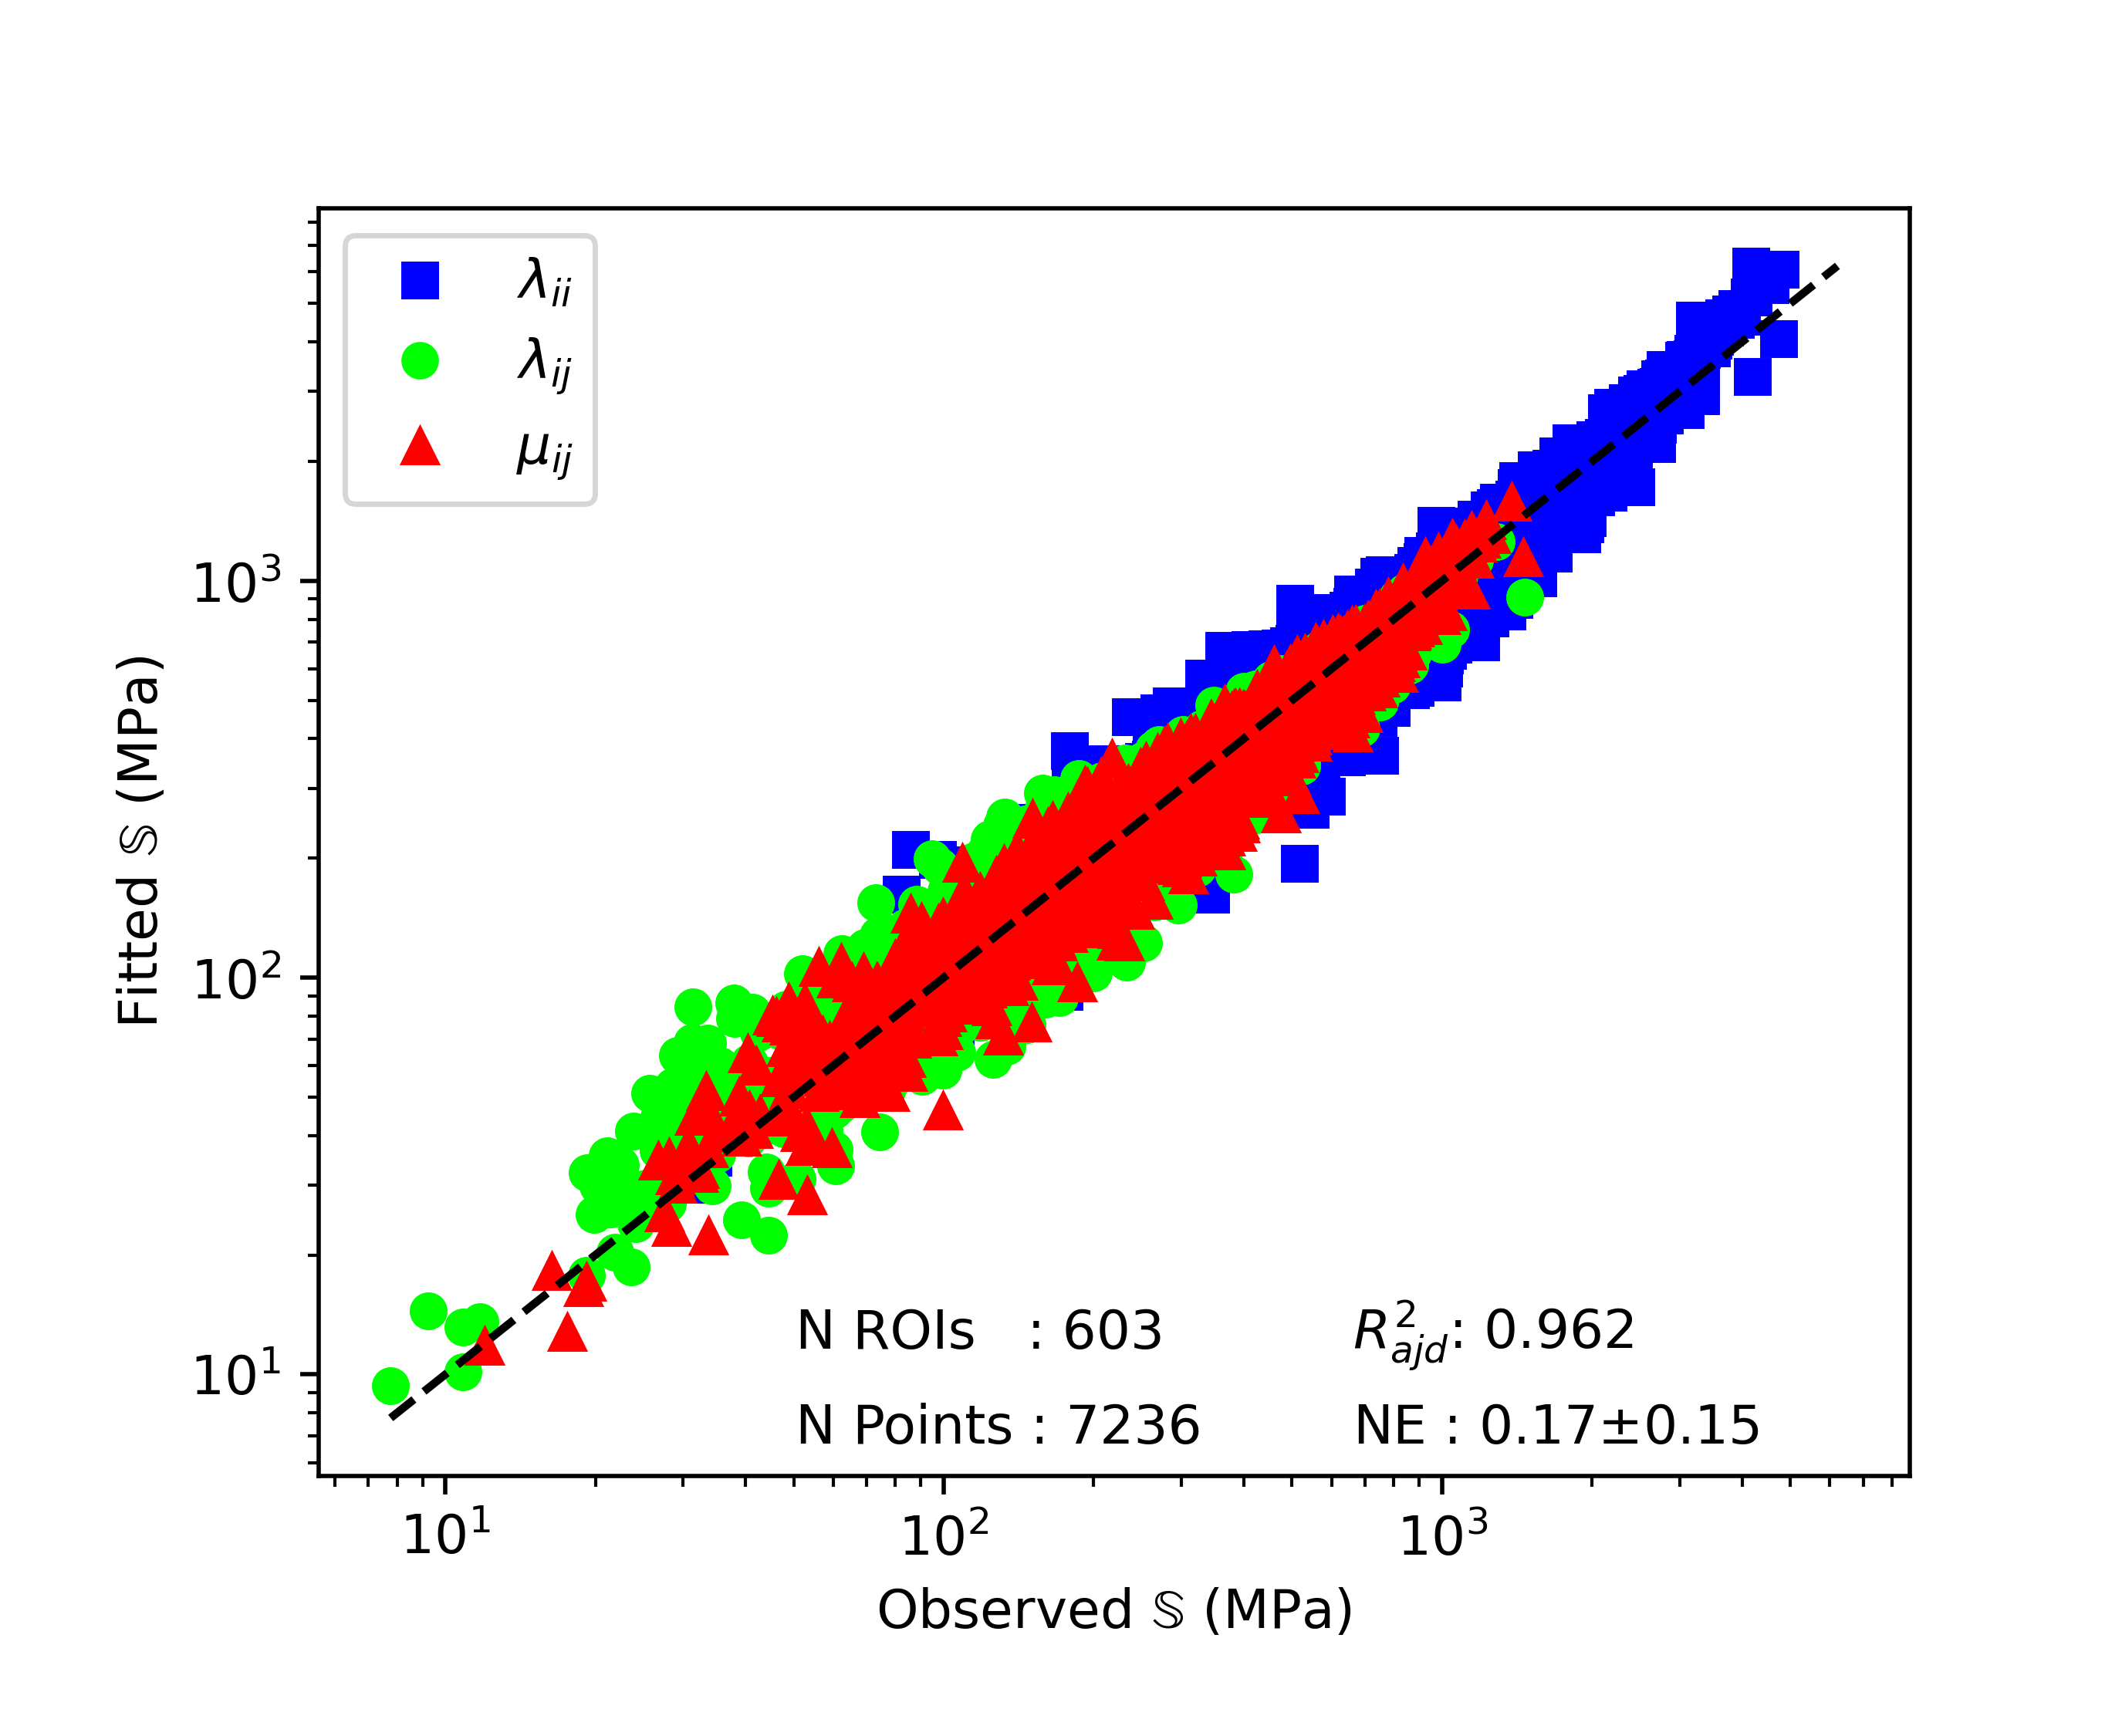
\includegraphics[width=\linewidth]{../_Results/StandardModel_Trabecular}
	% 		\caption{Standard model}
	% 	\end{subfigure}
	% 	\begin{subfigure}[b]{0.45\linewidth}
	% 		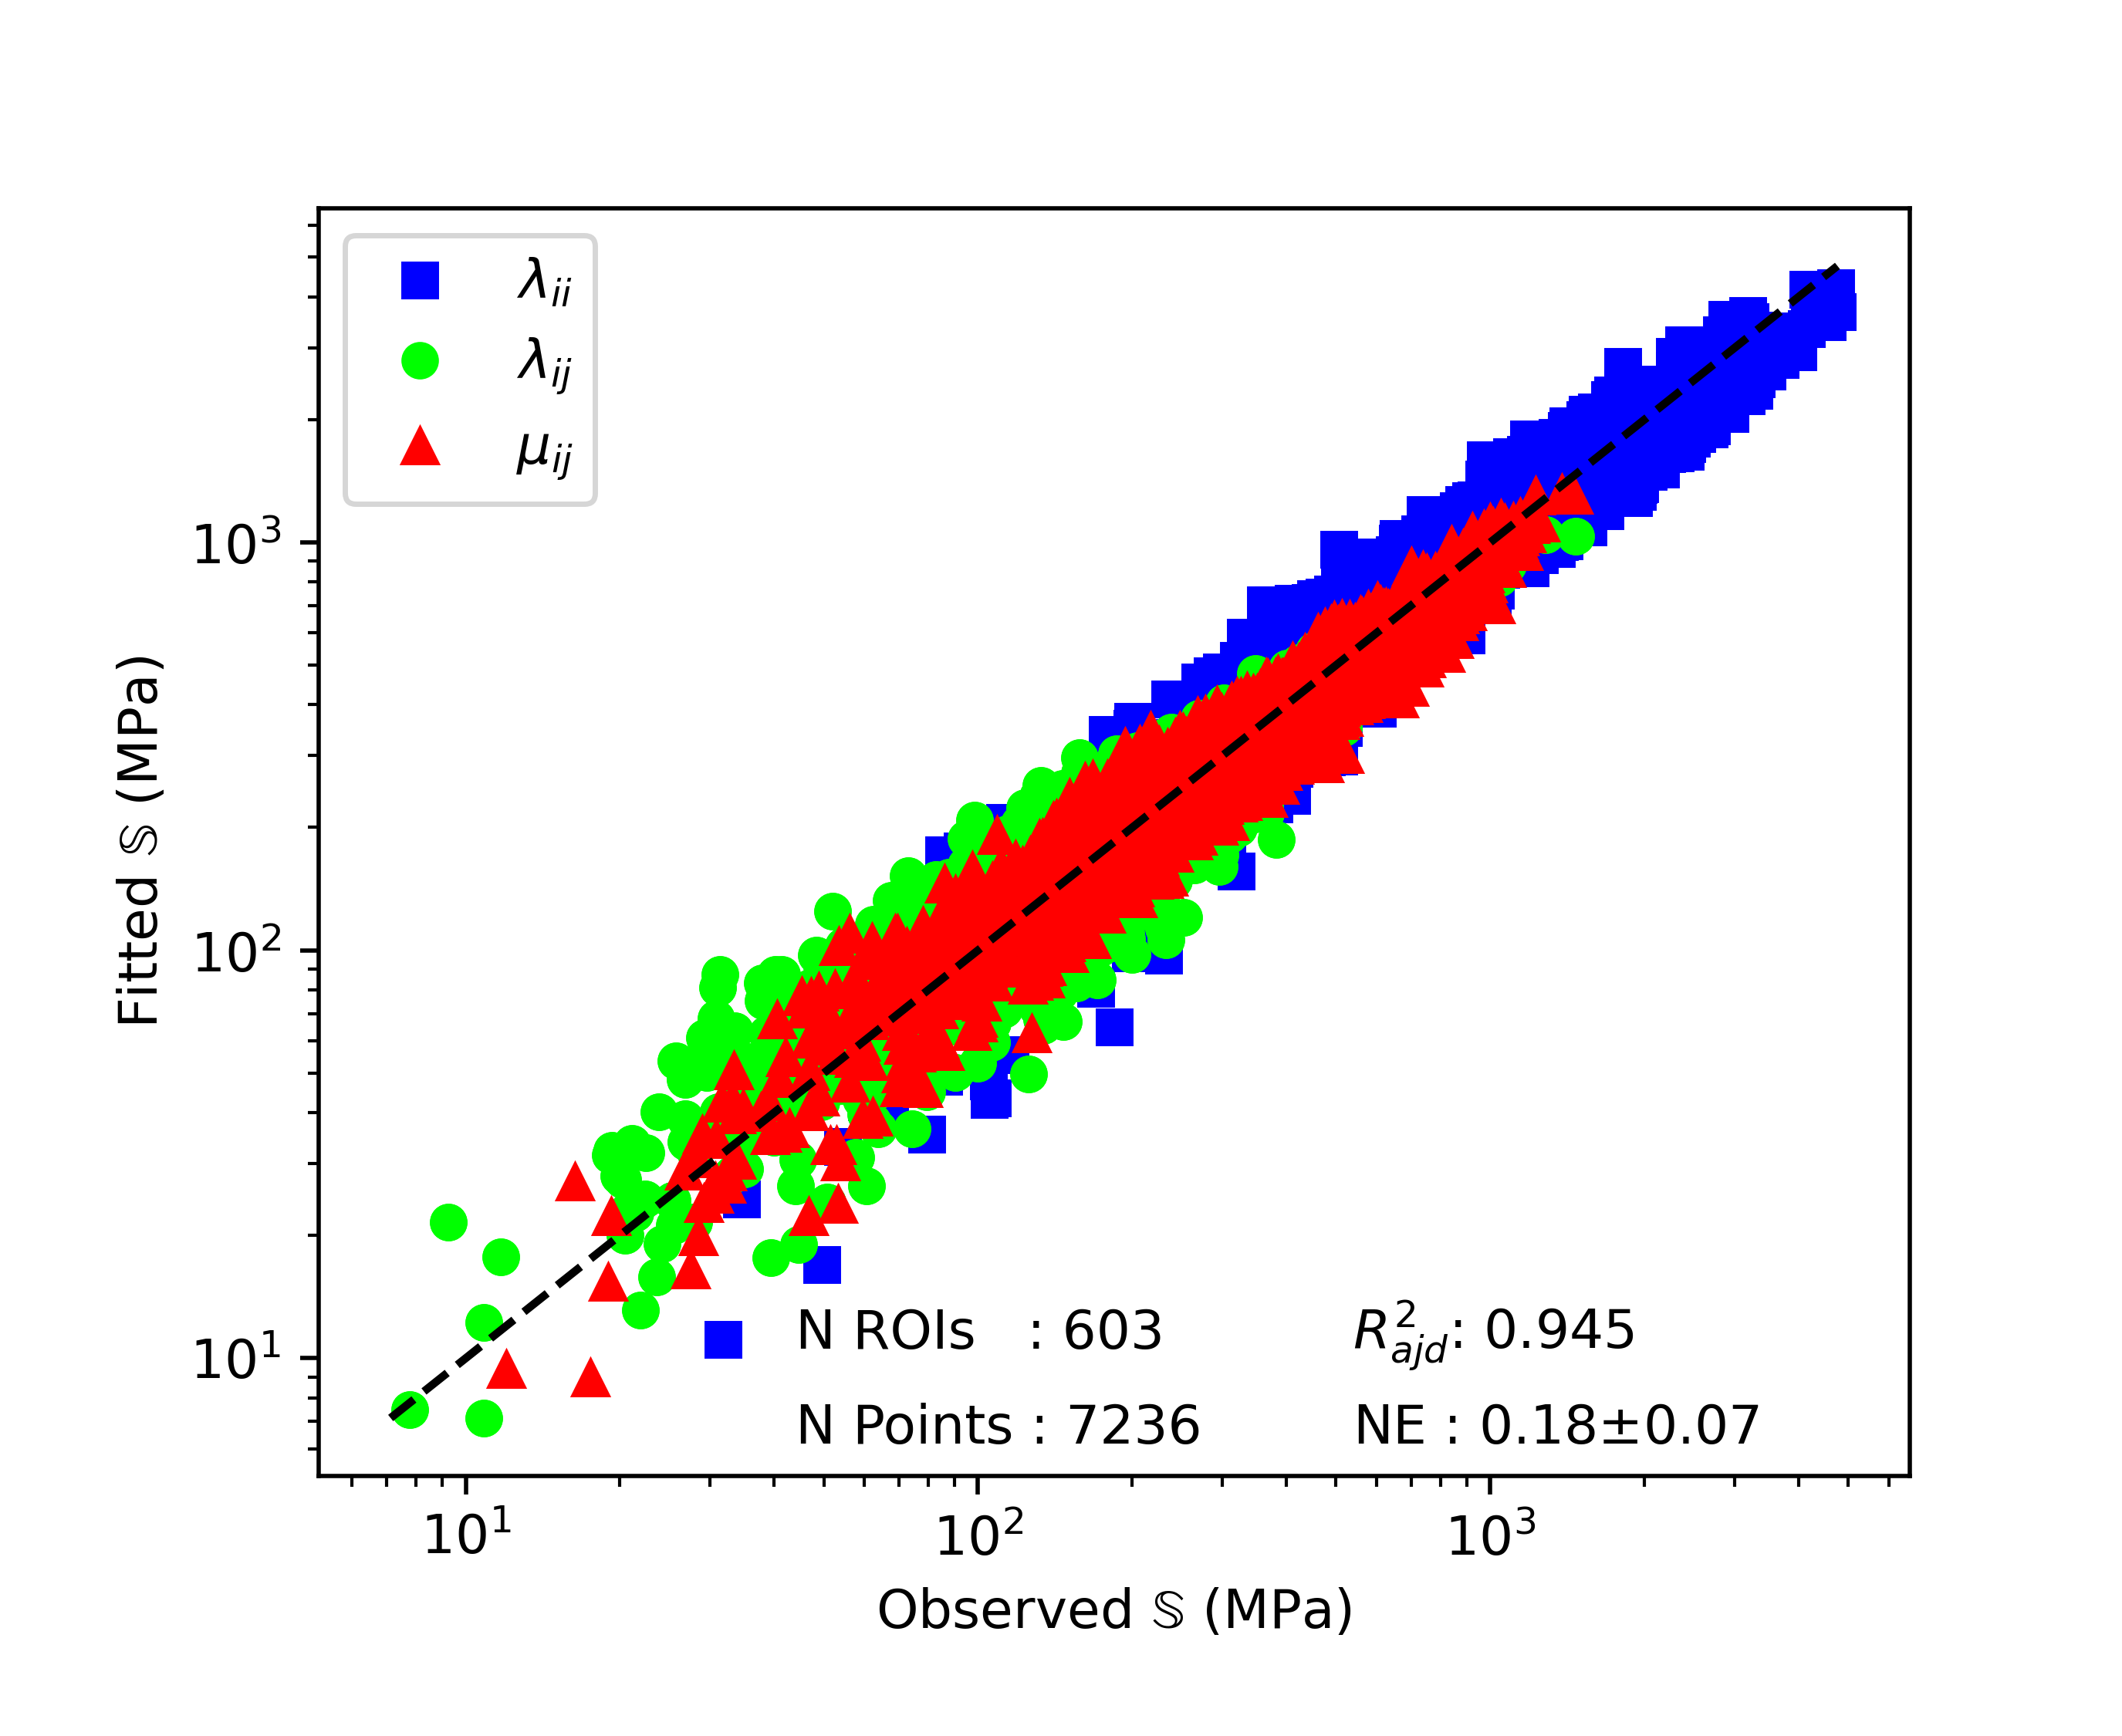
\includegraphics[width=\linewidth]{../_Results/ProposedModel_Trabecular}
	% 		\caption{Proposed model}
	% 	\end{subfigure}
	% 	\caption{Fit to trabecular data}
	% \end{figure*}

	% \begin{table*}[!h]
	% 	% \resizebox{\linewidth}{!}{%
	% 	\begin{tabular}{l|c|c|c|c|c|c|c|c|c|c}
	% 		Model & $\lambda_0$ & $\lambda_0$' & $\mu_0$ & $k_\lambda$ & $k_\mu$ & $l$ & $R^2_{adj}$ & NE \\
	% 		\hline
	% 		Standard & 8866 & 3223 & 2024 & 2.03 & 2.03 & 0.82 & 0.962 & 0.17 \\
	% 		Proposed & 7610 & 2768 & 1739 & 1.845 & 1.846 & -0.46 & 0.945 & 0.18 \\
	% 		\hline
	% 	\end{tabular}
	% \end{table*}


	\clearpage
	\subsection{Comparison to RUS}

	\begin{figure}[!h]
		\centering
			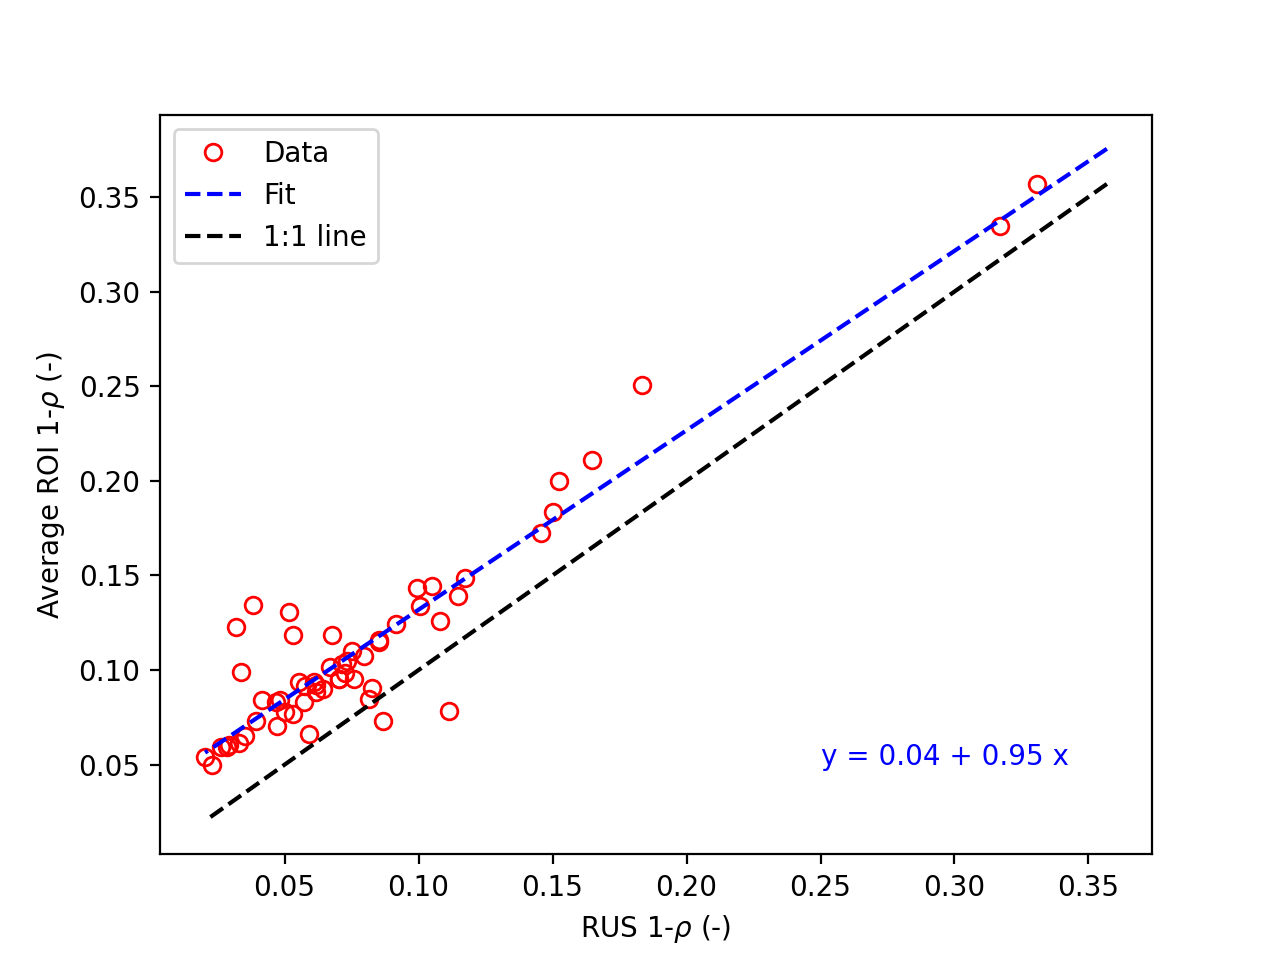
\includegraphics[height=\linewidth]{../_Results/Cortical/ExpSim_Rho}
			\caption{Average ROI porosity vs porosity from Cai et al.}
	\end{figure}

	\begin{figure}[!h]
		\centering
			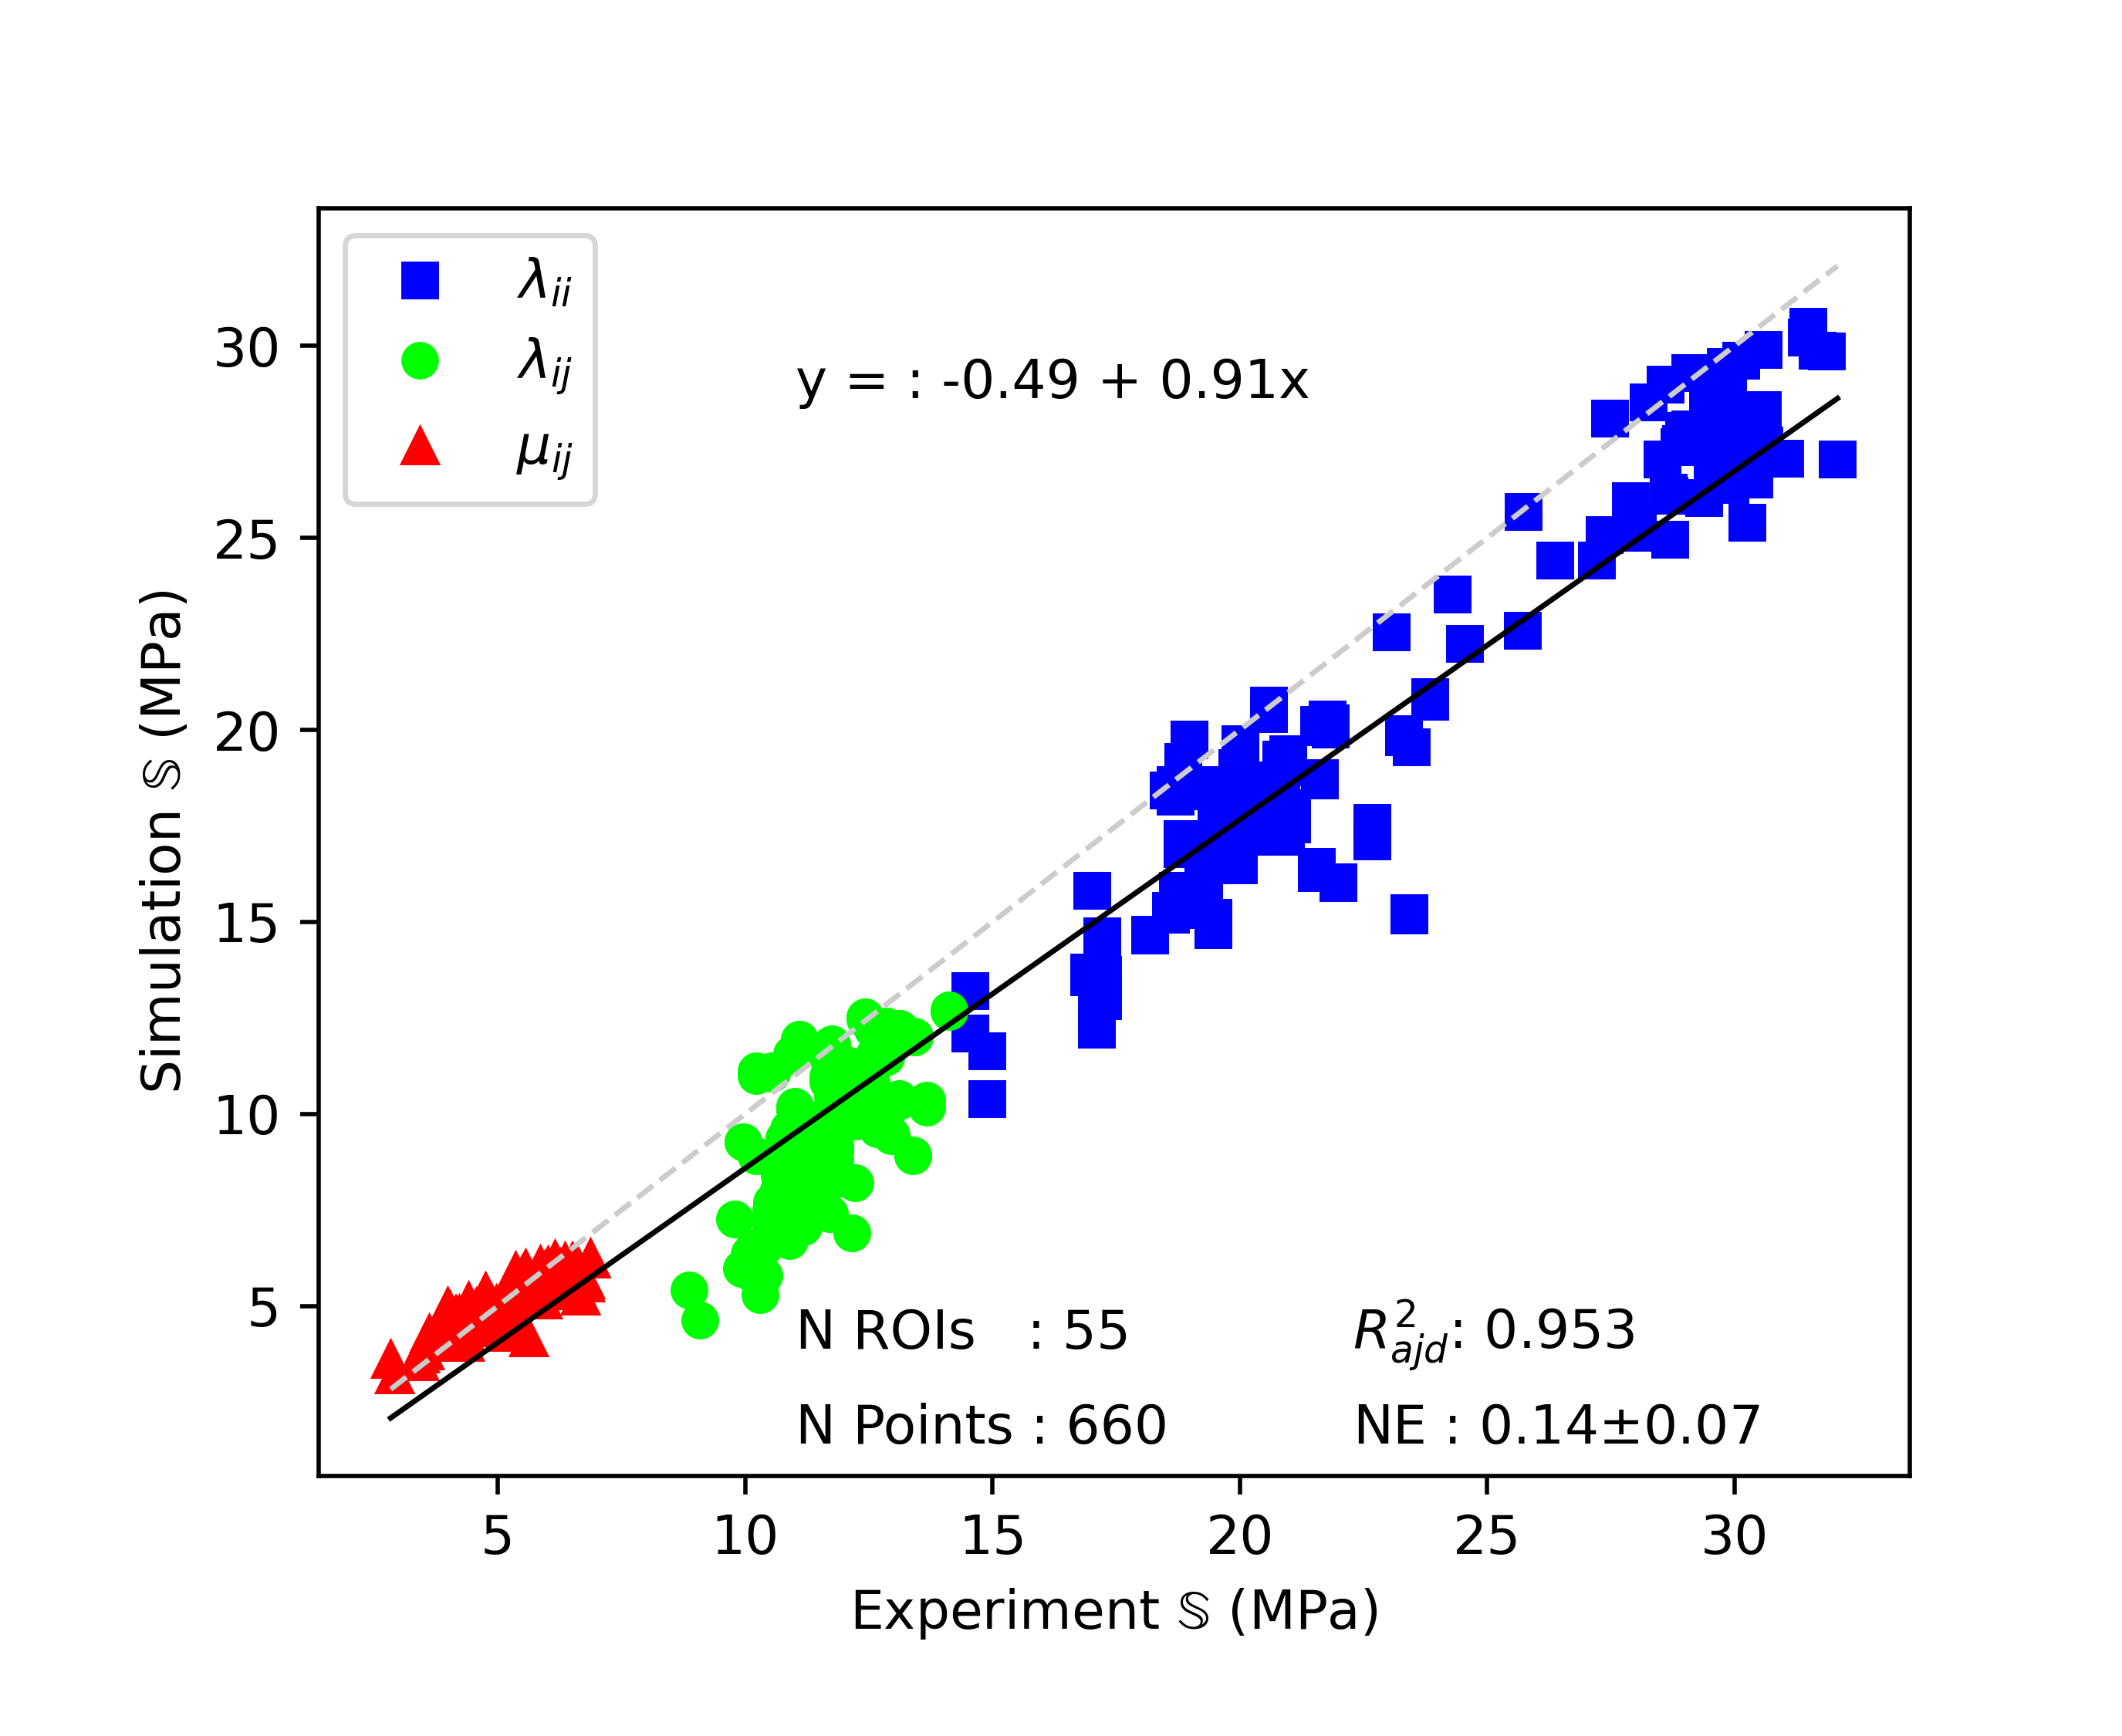
\includegraphics[height=\linewidth]{../_Results/Cortical/ExpSim_S}
			\caption{Simulation vs experimental stiffness tensor components}
	\end{figure}

	\begin{figure*}
		\centering
		\begin{subfigure}[b]{0.45\linewidth}
			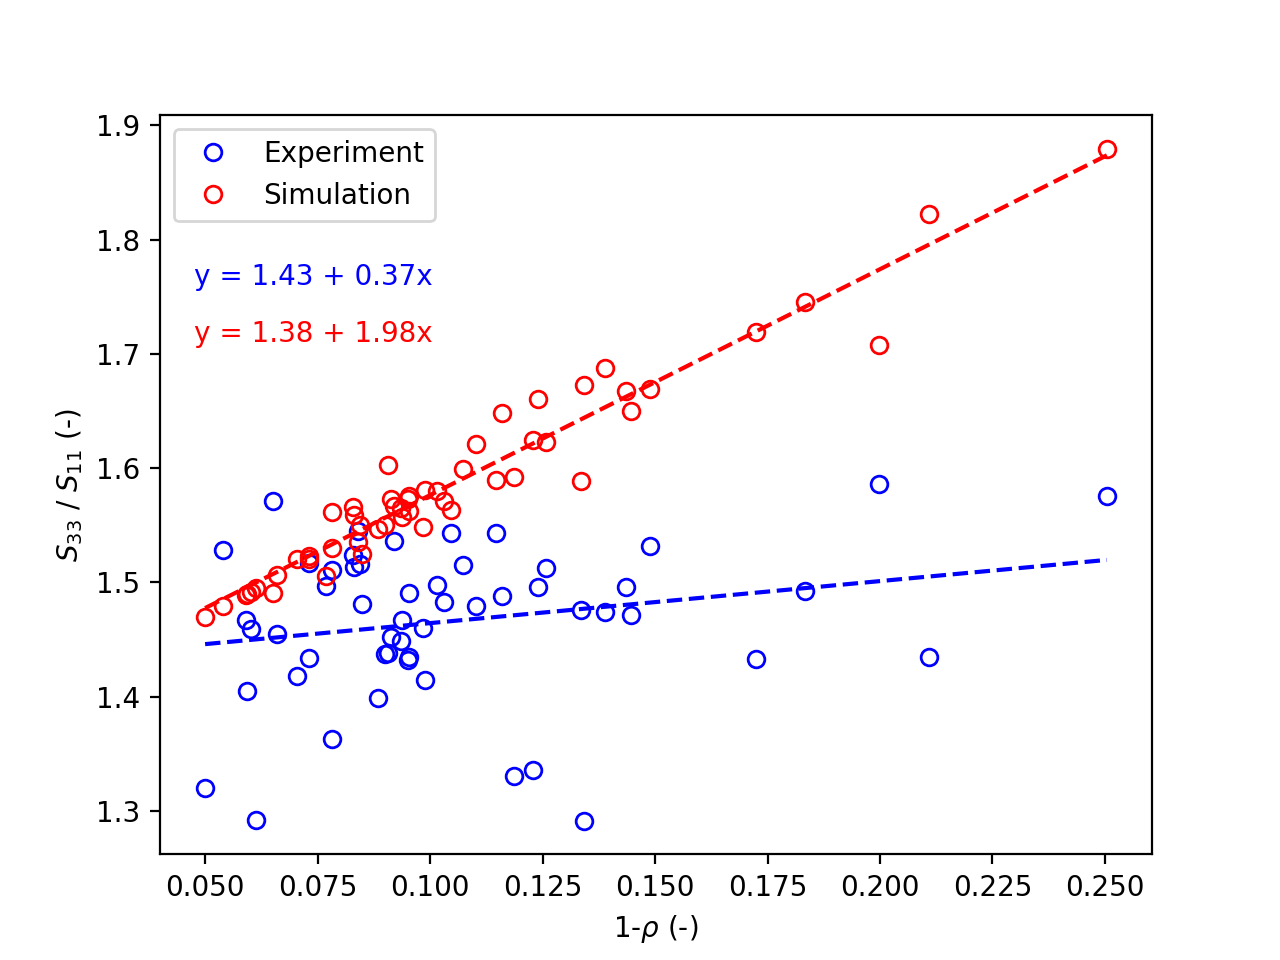
\includegraphics[width=\linewidth]{../_Results/Cortical/ExpSim_AniS}
			\caption{Stiffness ratio}
		\end{subfigure}
		\begin{subfigure}[b]{0.45\linewidth}
			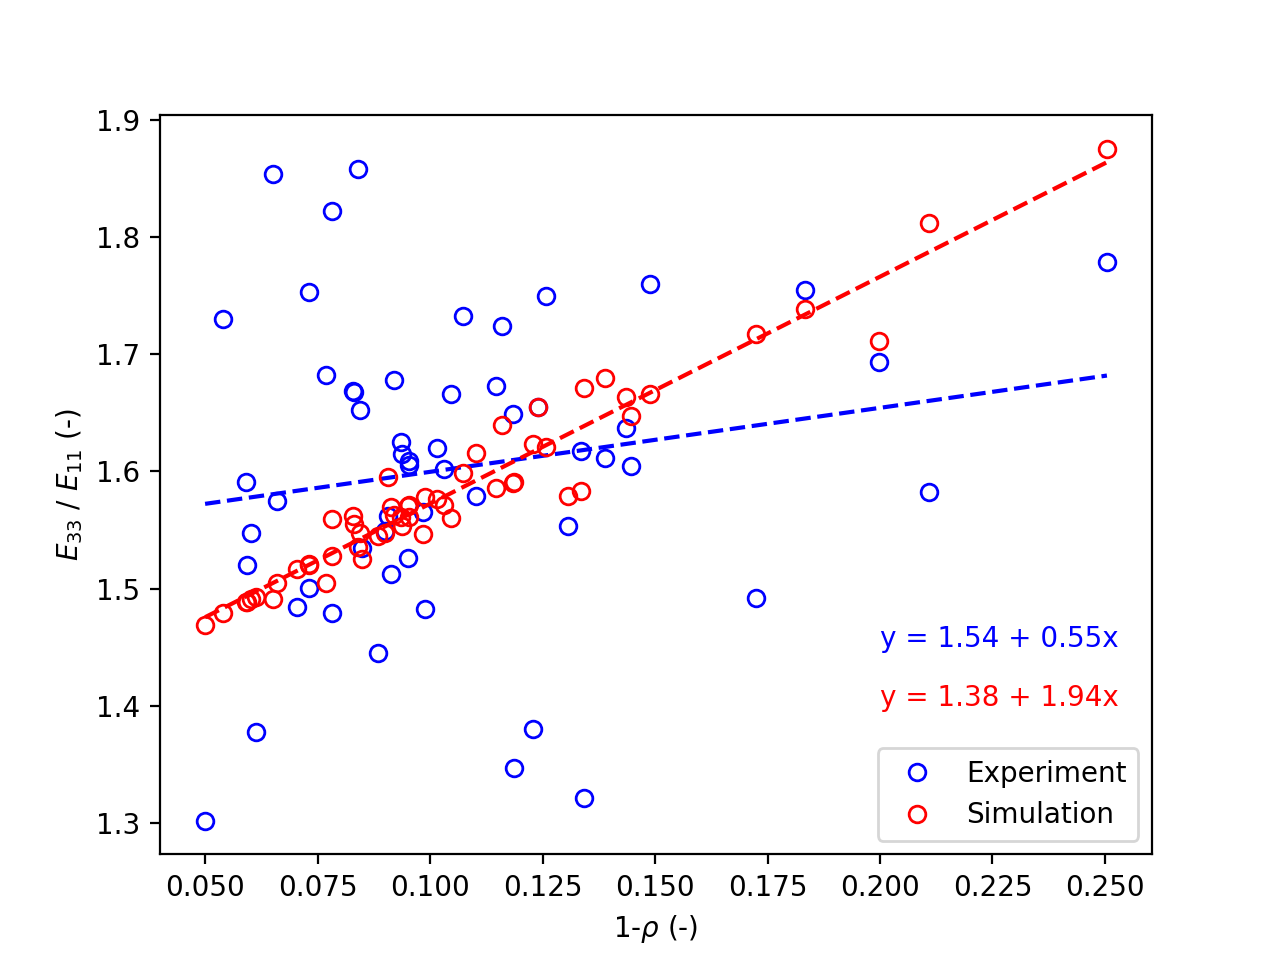
\includegraphics[width=\linewidth]{../_Results/Cortical/ExpSim_AniE}
			\caption{Young's moduli ratio}
		\end{subfigure}
		\caption{Degree of anisotropy}
	\end{figure*}

	%
	%
	%
	% DISCUSSION
	%
	%
	%
	
	\clearpage
	\section{Discussion and Conclusion}
	
	%
	%
	%
	% ACKNOWLEGMENTS
	%
	%
	%
	
	\section*{Declaration of competing interest}
	We wish to confirm that there are no known conflicts of interest associated with this publication and there has been no significant financial support for this work that could have influenced its outcome.
	
	\section*{Funding}
	This work was funded by the Swiss National Science Foundation (SNSF), grant number 200365.

	\section*{Data availability statement}
	The data that support the findings of this study are available on request. The data are not publicly available due to privacy/ethical restrictions. The scripts used for the analyses performed in the present study are available on Github: \url{https://github.com/artorg-unibe-ch/FABTIB}
	
	\section*{Research ethics}
	We further confirm that any aspect of the work covered in this manuscript that has involved human patients has been conducted with the ethical approval of all relevant bodies and that such approvals are acknowledged within the manuscript.
	
	\section*{CRediT author statement}
	\textbf{Mathieu Simon:} Data Curation, Formal analysis, Investigation, Methodology, Software, Visualization, Writing - original draft.
	\textbf{Philippe Zysset:} Conceptualization, Funding acquisition, Methodology, Project administration, Resources, Supervision, Validation, Writing - review and editing.
	
	%
	%
	%
	% Bibliography
	%
	%
	%

	% \clearpage
	% Loading bibliography database
	\nocite{*}
	\bibliographystyle{BibStyle}
	\bibliography{Bibliography}

	% \bibliographystyle{elsarticle-num} 

	% \begin{thebibliography}{65}
	% \expandafter\ifx\csname natexlab\endcsname\relax\def\natexlab#1{#1}\fi
	% \providecommand{\url}[1]{\texttt{#1}}
	% \providecommand{\href}[2]{#2}
	% \providecommand{\path}[1]{#1}
	% \providecommand{\DOIprefix}{doi:}
	% \providecommand{\ArXivprefix}{arXiv:}
	% \providecommand{\URLprefix}{URL: }
	% \providecommand{\Pubmedprefix}{pmid:}
	% \providecommand{\doi}[1]{\href{http://dx.doi.org/#1}{\path{#1}}}
	% \providecommand{\Pubmed}[1]{\href{pmid:#1}{\path{#1}}}
	% \providecommand{\bibinfo}[2]{#2}
	% \ifx\xfnm\relax \def\xfnm[#1]{\unskip,\space#1}\fi
	% %Type = Article
	% \bibitem[{Bala and Seeman(2015)}]{Bala2015}
	% \bibinfo{author}{Bala, Y.}, \bibinfo{author}{Seeman, E.}, \bibinfo{year}{2015}.
	% \newblock \bibinfo{title}{Bone's material constituents and their contribution
	% 	to bone strength in health, disease, and treatment}.
	% \newblock \bibinfo{journal}{Calcified Tissue International 2015 97:3}
	% 	\bibinfo{volume}{97}, \bibinfo{pages}{308--326}.
	% \newblock \URLprefix
	% 	\url{https://link.springer.com/article/10.1007/s00223-015-9971-y},
	% 	\DOIprefix\doi{10.1007/S00223-015-9971-Y}.
	
	% \end{thebibliography}

	%
	%
	%
	% Appendix
	%
	%
	%

	\clearpage
	\appendix
	
	
\end{document}